\documentclass{thesisreport}

\usepackage{caption}
\usepackage{subcaption}
\usepackage{comment}

\begin{document}

 \thispagestyle{empty}

\def\lskip{\vspace{0.5cm}}


\begin{tabular}{p{7cm}p{8cm}}
ÉCOLE CENTRALE DE NANTES
&
% EMARO students only
% \raggedleft FIRST YEAR INSTITUTION	
\end{tabular}

\vspace{2cm}

% CORO-IMARO students
\begin{center} \large\sc MASTER CORO-IMARO\\ \normalsize{``CONTROL and ROBOTICS''} \end{center}

% EMARO students
%\begin{center} \large\sc MASTER ERASMUS MUNDUS \\ \normalsize{EMARO+ ``European Master in Advanced Robotics''} \end{center}


\begin{center}
	2016 / 2017\\
	\lskip
	Master Thesis Report % or bibliography report
	\lskip
	
	Presented by \lskip 
	
	Student Name \lskip
	
	On Date \lskip\lskip
	
	{\Large \textbf{The title of the master thesis}}
	
	\vfill

Jury \lskip
		
	\end{center}
	


\begin{tabular}{p{3cm}p{7cm}p{5cm} }
 % President: & Name & Position (Institution) \\ & & \\     % for final defense only (not bibliography)
 Evaluators: & Name & Position (Institution) \\
	      & Name & Position (Institution) \\ 
	      & Name & Position (Institution) \\ & & \\  & & \\ 
  Supervisor(s):  & Name & Position (Institution) \\
		  & Name & Position (Institution) \\
% EMARO students only
%(EMARO)  & Co-supervisor from M1 & Position, M1 institution 
\end{tabular}

\lskip

\begin{flushleft}
 Laboratory: Laboratoire des Sciences du Numérique de Nantes LS2N
\end{flushleft}

\newpage
\thispagestyle{empty}
\null
\newpage
\addtocounter{page}{-1}
\pagestyle{fancy}
  
 
  \section*{Abstract}
Within the rapidly growing aerial robotics market, one of the most substantial challenges in the quadrotor community is performing aggressive maneuvers, especially multi-flip maneuvers.  A proper physical definition of the issue is not addressed by the current approaches in the field and several key aspects of this maneuver are still overlooked.
It can be shown, in particular, that making a flip with a quadrotor means crossing the parallel singularity of the dynamic model. The aim of the master thesis is to explore the possibility of defining aggressive trajectories for quadrotors on the basis of their dynamic model degeneracy analysis and to adapt various strategies to control the robot in a closed loop. In addition, the possibility to perform the aggressive maneuver in constrained environments will also be investigated.
Therefore, the analysis will be extended from the previous studied to create general feasible trajectories that will allow quadrotors to perform aggressive flip maneuvers while passing through a constrained environment and while guaranteeing a satisfactory degree of robustness to the uncertainties of the dynamic model.

 
 \newpage
 
 \section*{Acknowledgements}


I would like to express my special thanks and gratitude to my supervisors Dr. Sébastien Briot and Dr. Isabelle Fantoni who gave me the  opportunity to work on this wonderful project which encapsulates control theory, dynamics and quadrotors. This project has allowed me to perform research on all of these topics and I am now more knowledgeable thanks to my supervisors. Moreover, I would like to thank them for believing in my capabilities and for me the confidence when I needed it. \\\\
Secondly, I would also like to thank Dr. Ina Taralova for providing me with the valuable knowledge to create a proper bibliography. \\\\
I would like to thank my patient and understanding girlfriend Glysa, who has been with me for more than 5 years. Thank you for all the love, support and comfort that you have given me in these stressful 2 years. I hope that this Master degree will allow us to have a better future together. \\\\
I would like to thank my family as well: my parents Naji and Yolla, my sister Rebecca, my uncle and his wife Fadi and Lara and my aunt Bernadette. They have provided me with the emotional and economical support from the very beginning and they gave me the opportunity to travel and study for this Master degree. They have always been proud and encouraging. I would not be here if it wasn't for them.

 
 \newpage
 
 
 \section*{Notations}
 
 \newpage
 
  \section*{Abbreviations}

 \newpage
 
 \listoffigures
 
\listoftables
 
 \tableofcontents
 
 
 \chapter*{Introduction}
 \addcontentsline{toc}{chapter}{Introduction}	 % non-numbered chapters do not appear in table of contents by default
 	The aim of this section is to provide a general summary of the robotic robotic platform that is used for this master thesis and to illustrate the main objective of the research work.
In specific, in the sections below, quadrotors and parallel robots are briefly presented.


 
 
 \section*{The quadrotor platform}

A quadrotor is a type of unmanned aerial vehicle with four rotors and six degrees of freedom. Typically, drones have a small size and low inertia which allows it to be controller by simple flight control systems. It is typically designed in a cross-configuration such that the electronics are held in the center of the platform and the rotors are placed at the borders.
An example of a real quadrotor, namely the DJI Phantom, is shown in fig. \ref{fig:drone}. The quadrotor is typically built in a way such that a pair of opposite rotors rotate clockwise, whereas the other pair of rotors rotates in counter-clockwise.
The attitude and the position of the drone are controlled by changing the spinning speed of the rotors. An example is shown in figure \ref{fig:propeller_directions}.



\begin{figure}[h]
     \centering
     \begin{subfigure}[b]{0.45\textwidth}
         \centering
         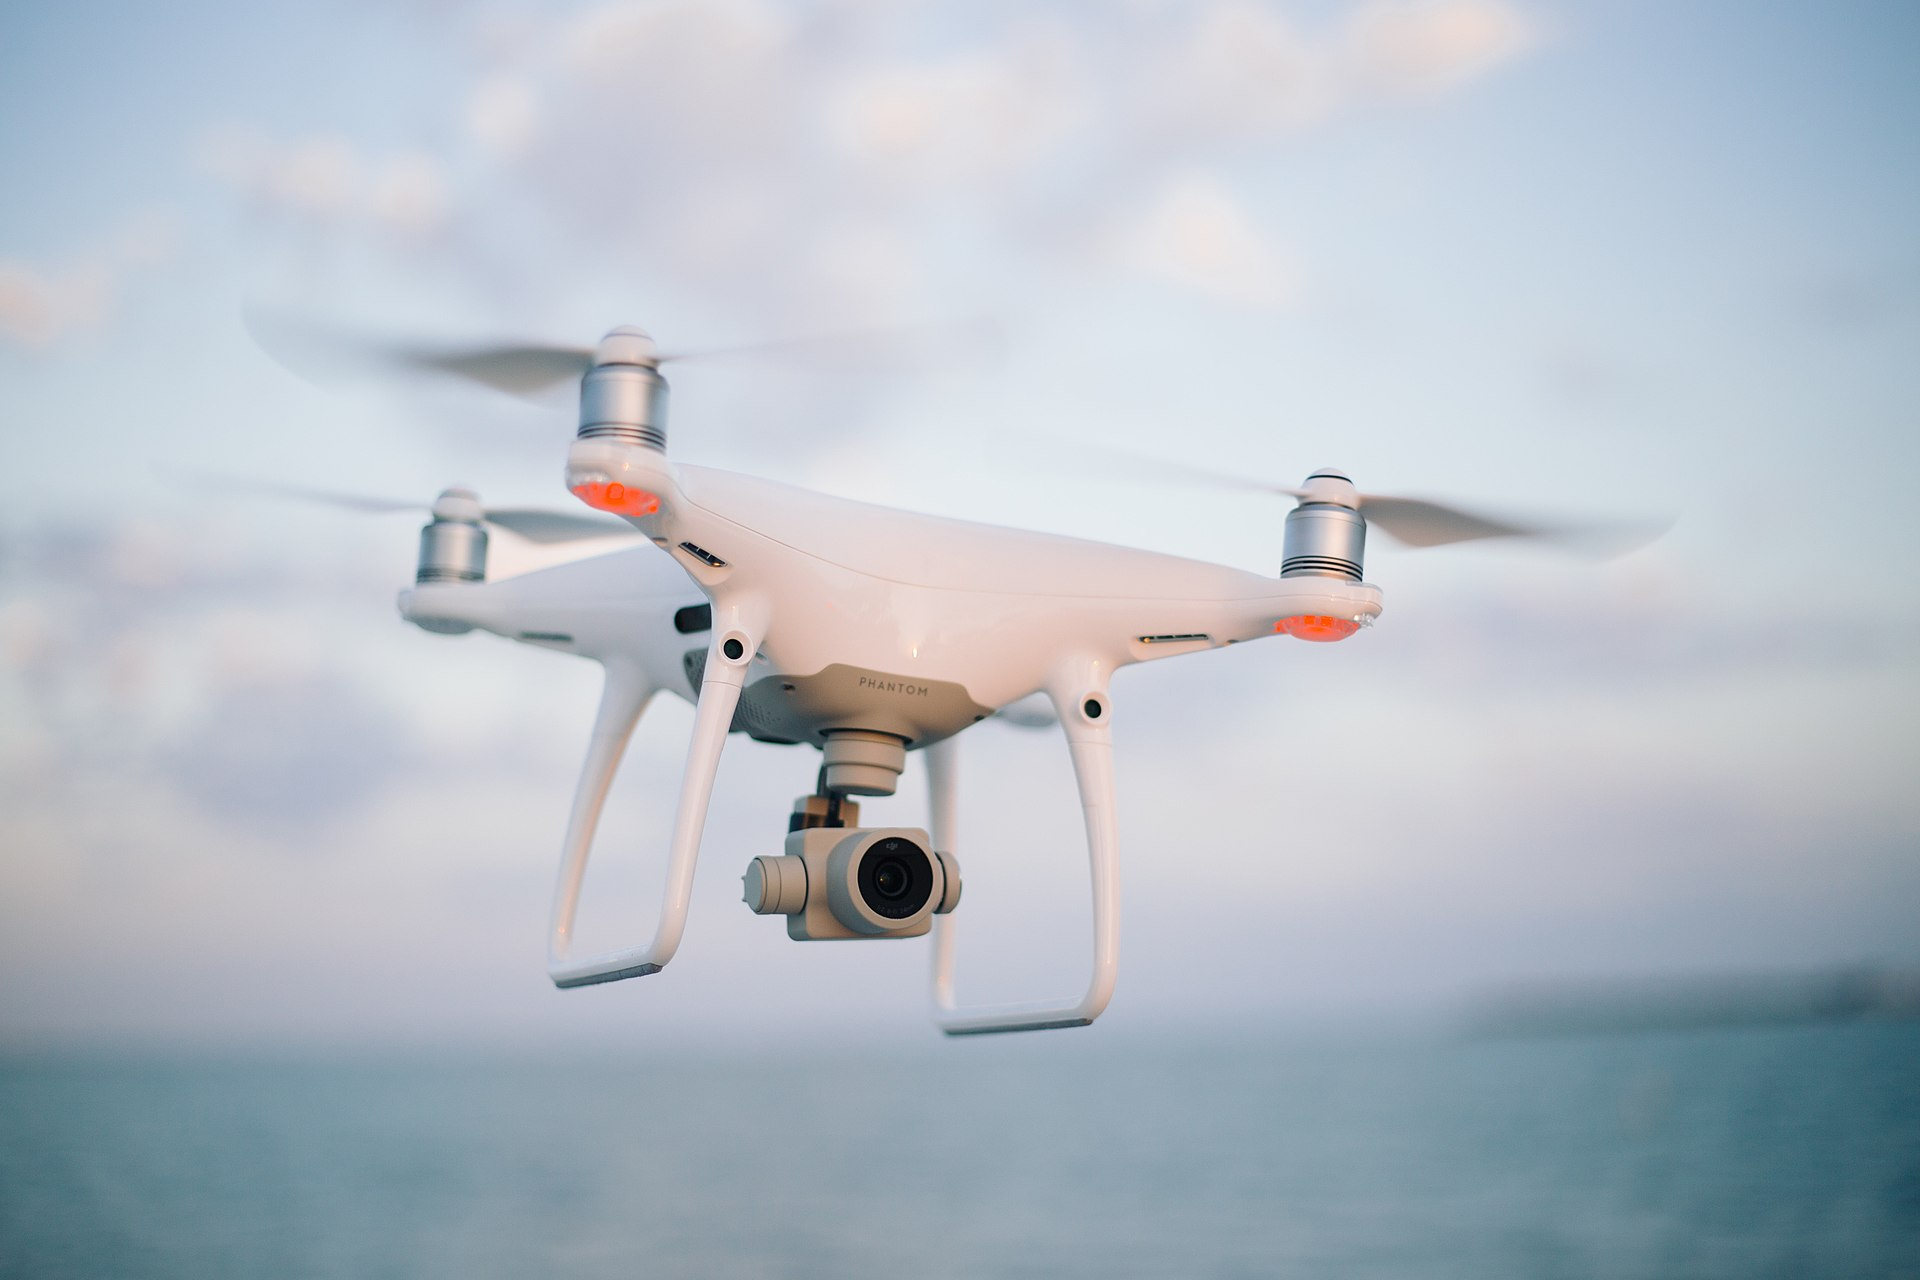
\includegraphics[width=\textwidth]{Images/Introduction/drone}
    \caption{A DJI Phantom quadcopter (UAV)}
         \label{fig:drone}
     \end{subfigure}
     \hfill
     \begin{subfigure}[b]{0.45\textwidth}
         \centering
         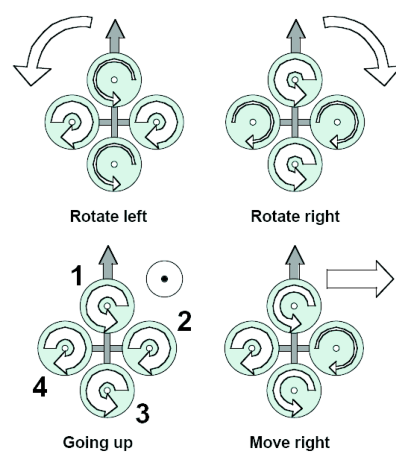
\includegraphics[width=0.6\textwidth]{Images/Introduction/propeller_direction.svg}
         \caption{Typical quadrotor configuration The width of the arrows is proportional to the angular speed of the propellers.\cite{Bouabdalla2007}}
         \label{fig:propeller_directions}
     \end{subfigure}
        \caption{A commercial quadrtotor platform, with a typical quadrotor configuration.}
        \label{fig:three graphs}
\end{figure}

The distinctive mechanical design of the quadrotor permits the actuation system to control all of the six degrees of freedom, even though it is under-actuated. This is due to the fact that the rotational and translational dynamics are tightly coupled. Thus, all the translational and rotational motions can be carried off by properly controlling the magnitude and direction of the spinning speed of the rotors.   

\pagebreak

Over the last few years, quadrotors have gained a large popularity in academia and in the industry. This is due to several reasons, such as: 

\begin{enumerate}

    \item Quadrotors are very simple to design and they can be easily assembled using relatively cheap components.  
    \item As quadrotors became more and more affordable and dependable, the number of quadrotors real-world applications has grown significantly. They are being used for aerial photography, agriculture, surveillance, inspection tasks, in addition to many other uses as well. 
    \item Quadrotors are quite agile and maneuverable during flight. Especially when compared to other types of unmanned aerial vehicles (UAVs). 
    
\end{enumerate}

However, on the main challenges in the quadrotors community is the capability to design control and planning methods that will allow the quadrotors to carry out aggressive maneuvers.  The fast dynamics associated with typically small dimensions of such agile quadrotors, in addition to several aerodynamic effects that will become important during aggressive flight maneuvers, are just a few of the main problems that are faced during the system control design. Moreover, accurate tracking of the provided trajectory is a very big issue in the case of aggressive maneuvers when the rotors are commanded high speeds and accelerations, which will cause rotors to become saturated and may also cause delays.


 \section*{Parallel manipulators}

A parallel manipulator is a mechanical system that consists of two connected platforms, the fixed platform and the moving platform. The latter is linked to the fixed platform thanks to at least two serial chains that are working in parallel. When compared to serial manipulators, parallel manipulators are more accurate and rigid. In addition, the ability to install the motors next to the fixed platform is a very important feature for parallel manipulators. Moreover, parallel manipulators can be used in a wide variety of applications that demand precision and high payload combined with high speed.\cite{Parallel_Manipulators}

\begin{figure}[h]
     \centering
     \begin{subfigure}[h]{0.45\textwidth}
         \centering
         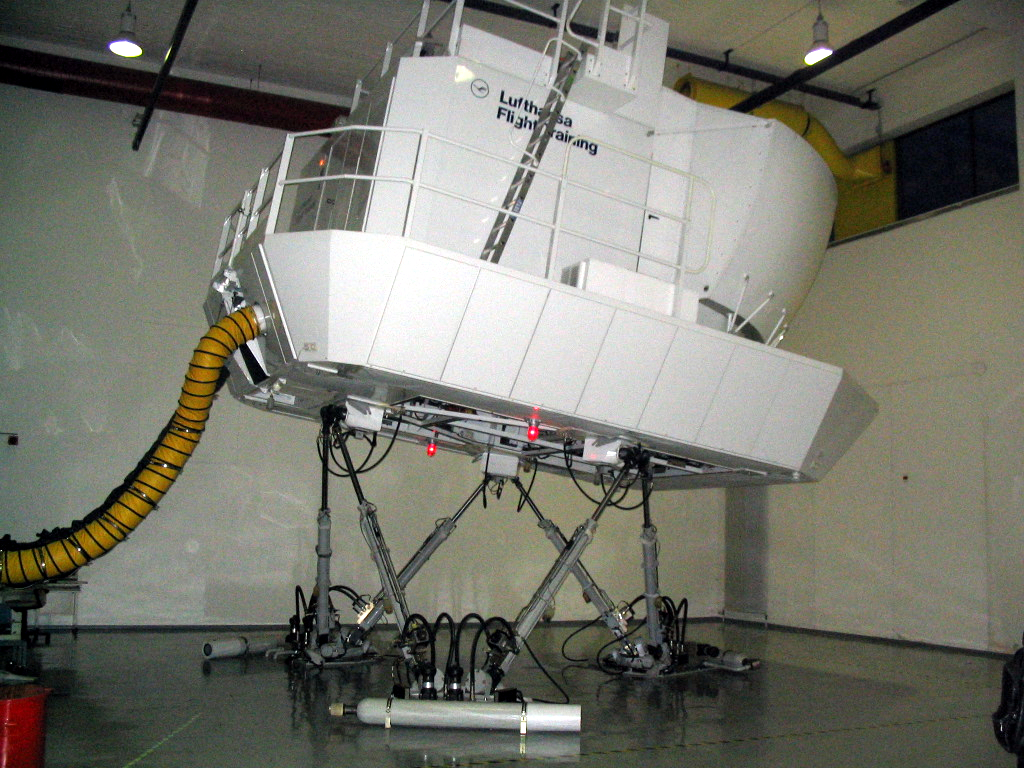
\includegraphics[width=0.7\textwidth]{Images/Introduction/GS}
    \caption[Caption for LOF]{Gough-Stewart used for a flight-simulator application.\protect\footnotemark}
         \label{GS}
     \end{subfigure}
     \hfill
     \begin{subfigure}[h]{0.45\textwidth}
         \centering
         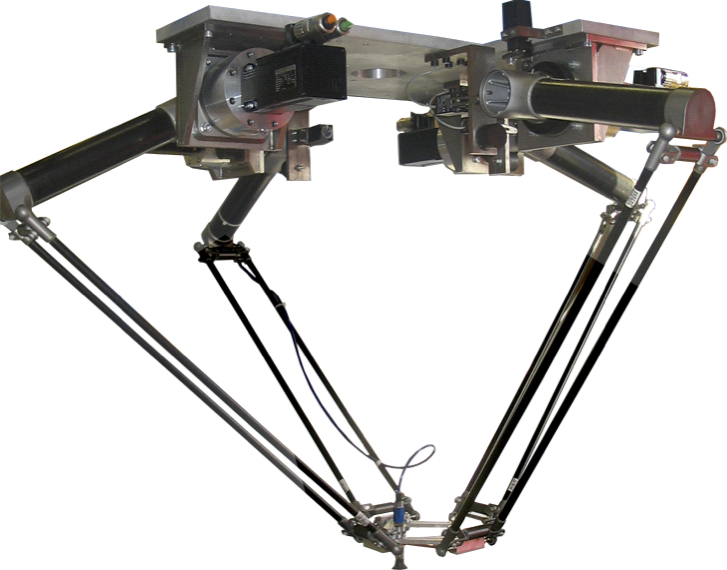
\includegraphics[width=0.7\textwidth]{Images/Introduction/PAR4}
         \caption[Caption for LOF]{The "PAR4" 4 degrees of freedom, high-speed, parallel robot prototype.\protect\footnotemark}
         \label{PAR4}
     \end{subfigure}
        \caption{Two examples of parallel robots.}
        \label{fig:three graphs}
\end{figure}




\footnotetext[1]{\url{https://en.wikipedia.org/wiki/Stewart_platform\#/media/File:Simulator-flight-compartment.jpeg}}
\footnotetext[2]{\url{https://en.wikipedia.org/wiki/Parallel_manipulator\#/media/File:Prototype_robot_parall\%C3\%A8le_PAR4.jpg}}


\pagebreak

However, parallel manipulators are subject to singularities, which can lead to big problems in the robot workspace in case they were not handled correctly. Thus, the study of the singular configuartions of parallel manipulators is very important. Because, even just before reaching a singularity, the performance of the parallel manipulator will decrease dramatically. Moreover, the robot may loose the ability of moving in a certain direction, gain uncontrollable motions and it the mechanism could even break. The main difference between serial and parallel manipulators is that singularity configurations may also appear inside the robot workspace (depending on the dimensions of the robot) and not just at the boundaries of the robot workspace, which can significantly decrease the area of the robot workspace.
As a result, many works have been developed by robotics researchers in order to allow parallel manipulator manipulators to safely cross these singularities by using trajectory planning and specific control methods.

\section*{The goal of this thesis}

This master thesis lies at the intersection of parallel robotics and aerial robotics. The two fields may seem very different from each other. However, quadrotors can be seen as a particular case of a parallel manipulator. 
In fact, a parallel manipulator is made up of a wrench system, applied by the robot limbs on the moving platform. And, this wrench system will define the motion of the moving platform. In the same manner, each propeller in a quadrotor can be considered as limb of a parallel robot and the moving platform to be controlled can be considered as the body of the drone. 
Specifically, the goal of this master thesis is to study a distinct class of aggressive maneuvers for quadrotors, namely multi-flip maneuvers. By doing multi-flip maneuvers, full rotations around one or more axes of the body of the quadrotor can be done. In addition, the quadrotor must also must also do the flips in a constrained environment.

\begin{figure}[h]
     \centering
     \begin{subfigure}[h]{0.45\textwidth}
         \centering
         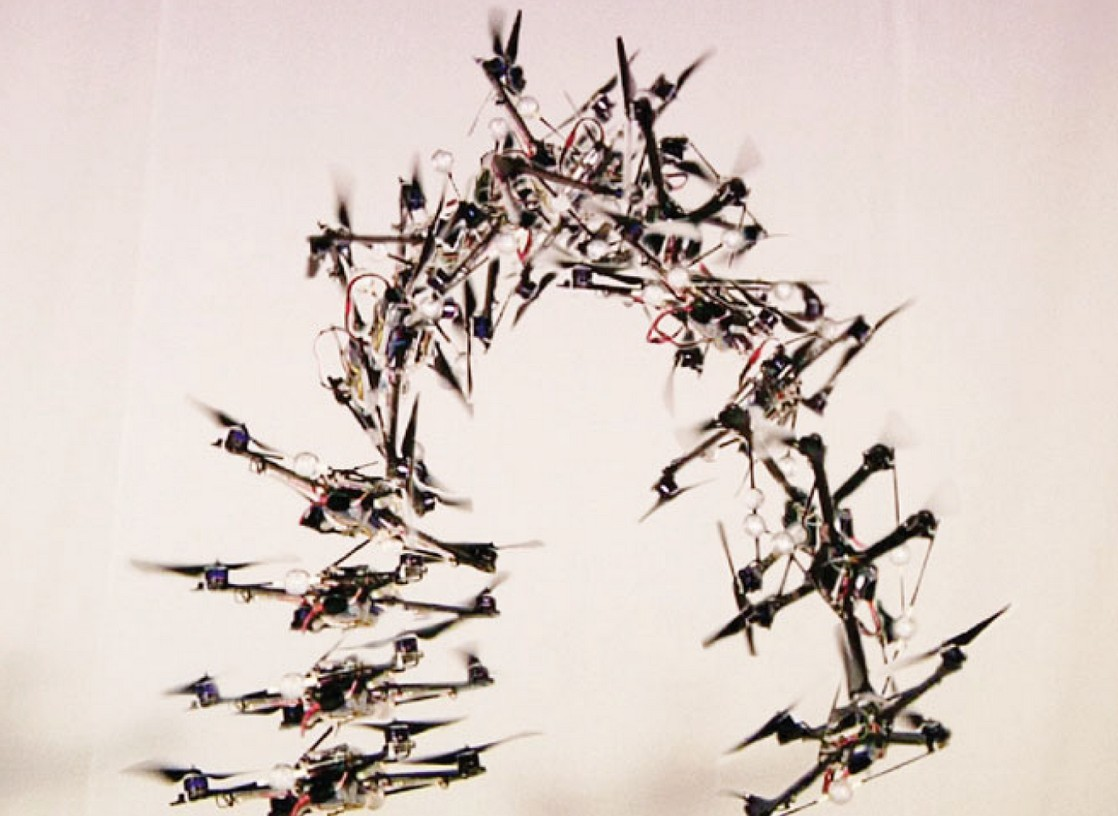
\includegraphics[width=0.9\textwidth]{Images/Introduction/flip}
    \caption{Quadrotor performing a triple flip.\cite{flip}}
         \label{triple_flip}
     \end{subfigure}
     \hfill
     \begin{subfigure}[h]{0.45\textwidth}
         \centering
         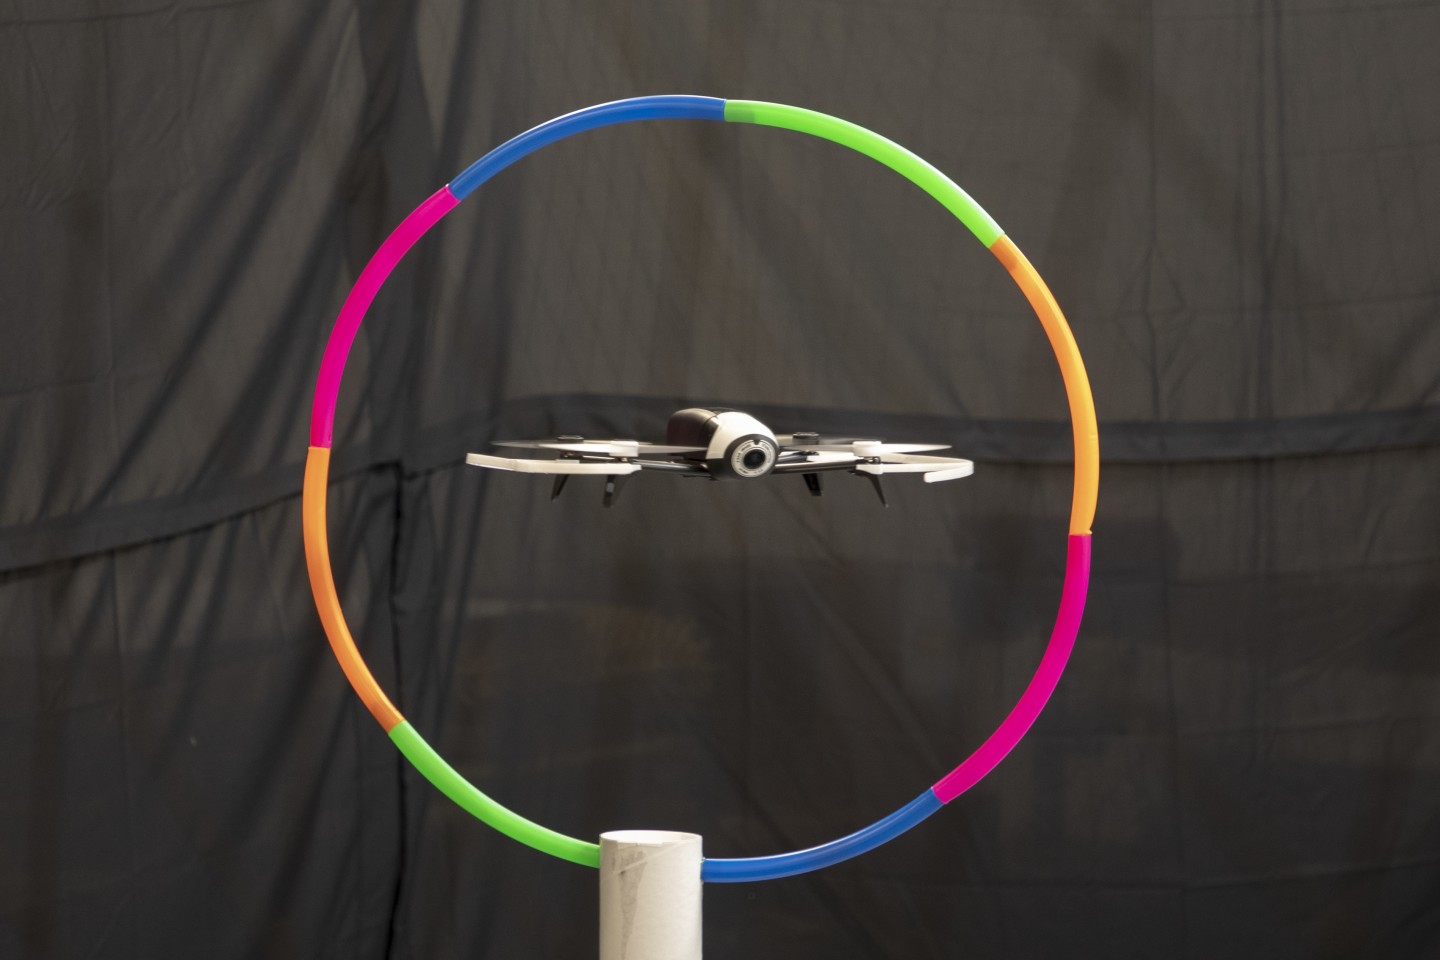
\includegraphics[width=\textwidth]{Images/Introduction/constrained_environment}
         \caption[Caption for LOF]{Quadrotor going though a loop.\protect\footnotemark[1]}
         \label{drone_hulahoop}
     \end{subfigure}
        \caption{Representation of the issues to be tackled in this master thesis.}
        \label{fig:three graphs}
\end{figure}

\footnotetext[1]{\url{https://newatlas.com/drones/muscle-signals-drone-control/\#gallery:2}}

\pagebreak

\section*{Outline of the work}

The rest of the bibliography is structured as follows:


\begin{itemize}
\setlength{\itemindent}{-.5in}
	\item [] \textbf{Chapter 1} is devoted to introduce the system modeling of quadrotors. Specifically, a simplified dynamic model of the quadrotor will be presented by using Euler-Lagrange formalism. Then, moving on from the simple dynamic model, a more detailed dynamic model will be presented by using the Newton-Euler formalism. Finally, the state-space model of the quadrotor will also be derived.

	\item [] \textbf{Chapter 2} provides an overview of state of the art in quadrotor control in addition to introducing the different potential control methods that can be used during the master thesis in order to properly control the quadrotor. 

	\item [] \textbf{Chapter 3} provides detailed explanations of how multi-flip maneuvers can be handled. Then, the link between a quadrotor performing a flip and a parallel robot crossing a singularity will be explained. In the end, a literature review is provided in order to show how the problem is tackled by different researches.

	\item [] \textbf{Chapter 4} is devoted to trajectory optimization. By using trajectory optimization, it will be possible to create feasible trajectories for quadrotors to perform the aggressive maneuvers in constrained environments.
	
\end{itemize}

\newpage

\chapter{System Modeling}
The goal of this chapter is to present the dynamic model of the quadrotor. The mathematical notation and the physics of the quadrotor platform are expressed using the Newton-Euler formalism. Then, the state-space model that will be coded on the controller of the quadrotor will be derived.

\section{Concepts and Generalities}
The dynamic model of the quadrotor will be derived based on the following assumptions:

\begin{itemize}
	\item The structure of the quadrotor is rigid.
	\item The structure of the quadrotor is symmetrical.
	\item The center of gravity (CoG) and the fixed frame at the center of the body are assumed to be coincident.
	\item The proppelers of the quadrotor are assumed to be rigid.
	\item The thrust and drag forces are assumed to be proportional to the square of the spinning speed of each propeller.
\end{itemize}
 
The helicopter is a complex mechanical system, it gathers many physical effects from the domain of mechanics and aerodynamics \cite{houston_2001}. Thus, all the significant effects including the gyroscopic effects must be considered in the modeling of the quadrotor. A small list of the most important effects that a helicopter is subject to \cite{Mullhaupt1999} are briefly described in table \ref{physical_effects}:

\begin{table}[h]
\caption{The main physical effects that the helicopter is subject to. }\label{physical_effects}
\centering
\setlength{\tabcolsep}{10pt} % Default value: 6pt
\renewcommand{\arraystretch}{1} % Default value: 1
\begin{tabular}{c c c}
\hline
\hline
Effect & Source & formulation \\
\hline
Aerodynamic effects & \shortstack{Rotation of propeller \\ Flapping of blades} & $C \Omega^2$\\
\hline
Inertial counter torques & \shortstack{Change in propeller \\ spinning speed} & $ J \dot{\Omega}$\\
Gravitational effect & Position of the center of mass & {} \\
\hline
Gyroscopic effects & \shortstack{Orientation change  \\ of the rigid body} & $ I \theta \psi$\\
 {} & \shortstack{Orientation change  \\ of the propeller plane} & $ J \Omega_r \theta,\phi$ \\
 \hline
Friction & All helicopter motions & $C \dot{\phi},\dot{\theta},\dot{\psi}$\\
\hline
\hline
\end{tabular}
\end{table}

\newpage 

 \section{Modelling with Euler-Lagrange Formalism} 
 The dynamics of the rotation of a simple quadrotor are modeled using the Euler-Lagrange Formalism in this section. A fixed frame $E$ for the world frame and body fixed frame $B$ for the quadrotor are considered as represented in figure \ref{coordinate_system_simple}. The orientation of the quadrotor frame in space is provided by a rotation $R$ from $B$ to $E$, where $R\in SO3$ is a $3 \times 3 $ rotation matrix.
 
 
 \begin{figure}[h]
 \centering
 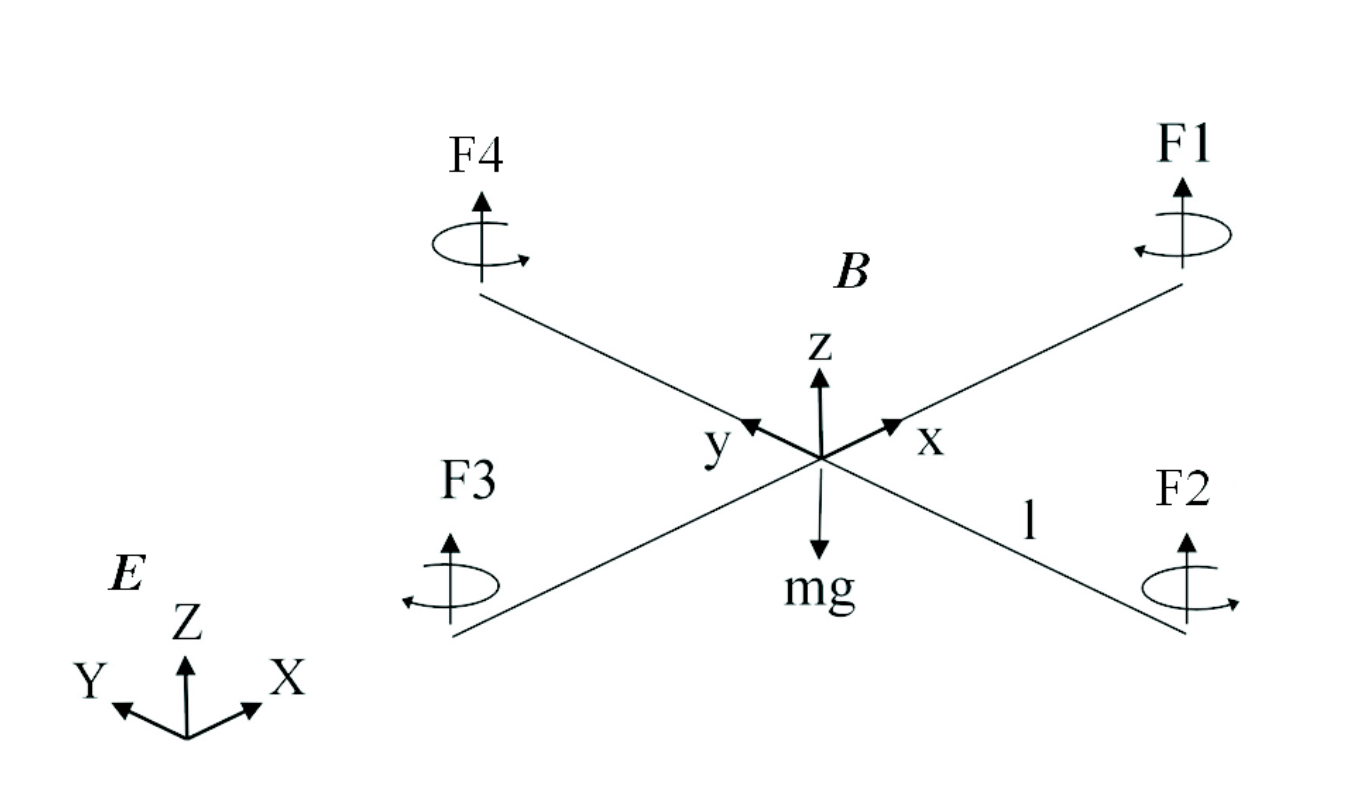
\includegraphics[width=0.5\textwidth]{Images/Modeling/Test_Bench}
 \caption{Coordinate system of a quadrotor. \cite{Bouabdalla2007}}
 \label{coordinate_system_simple}
 \end{figure}

\subsection{Kinematics} 
 
 For any point of the body frame of the quadrotor expressed in the fixed world frame, the following can be written ( c: $\cos$, s: $\sin$):   
 
 \begin{equation}\label{kinematics}
 \begin{cases}
 r_X= (c\psi c \theta ) x + ( c \psi s \theta s \phi  - s \psi c \phi) y + (c \psi s \theta c \phi + s \psi s \phi) z \\
 r_Y= (s\psi c \theta ) x + ( s \psi s \theta s \phi  + c \psi c \phi) y + (s \psi s \theta c \phi - c \psi s \phi) z \\
 r_Z= (-s \theta ) x + ( c \theta s \phi ) y + (c \theta c \phi) z \\
 
 \end{cases}
 \end{equation}

Thus, the velocities can be derived by differentiation \ref{kinematics}
, and the squared magnitude of the squared velocity can be expressed as follows for any point:

\begin{equation}\label{velocity_magnitude}
	v^2 = v_X^2 + v_Y^2 + v_Z^2\\
\end{equation} 

\subsection{Energy}

Assuming that the matrix of inertia is diagonal, then from equation \ref{velocity_magnitude},the expression of the kinetics energy can be calculated:

\begin{equation}\label{kinetic_energy}
T = \frac{1}{2} I_{xx}(\dot{\phi}-\dot{\psi} s \theta)^2 + \frac{1}{2} I_{yy}(\dot{\theta} c \phi + \dot{\psi} s \phi c \theta)^2 + \frac{1}{2} I_{zz}(\dot{\theta} s \phi - \dot{\psi} c \phi)^2
\end{equation}

Using the formula of the potential energy, equation \ref{kinetic_energy} can be expressed in the fixed world frame as: 

\begin{equation}\label{potential_energy}
V = \int xdm(x)(-g s \theta) + \int ydm(y)(g s \phi c \theta) + \int z dm (z) (g c \phi c \theta) 
\end{equation}

\newpage

\subsection{Equation of Motion}

By using the Euler-Lagrange formalism:


\begin{equation}
L = T - V \text{\hspace{0.5cm} ,\hspace{0.5cm}} \Gamma_i = \frac{d}{dt}\bigg(\frac{\partial L}{\partial \dot{q}_i}\bigg) - \frac{\partial L}{\partial q_i}
\end{equation}
 
 Where $L$ $\Gamma_i$ and $\dot{q}_i$ are the Lagrangian, the generalized forces and the generalized coordinates respectively. Thus, the equations of motion can be expressed as follows: 
 
 
 
 
 
\newpage  

 \section{State-space model}
  
  
 \chapter{Control of quadrotors}
 
 \section{General control architecture}
 
 \section{Model Predictive control}
 
 \section{Lyapunov Stability Analysis}
 
 \section{Sliding mode control}
 
 \section{Other types of control}
 
 \chapter{Multi-flips maneuver with quadrotors}
 
 \subsection{Quadrotor flip physics}
 
 \subsection{Link to parallel robots}
 
 \subsection{Control approaches for multi-flip maneuvers}
  
 \chapter{Trajectory optimization}

 
 


 

 
 
 \chapter*{Conclusion}
 \addcontentsline{toc}{chapter}{Conclusion}
 
 
 
 


 \addcontentsline{toc}{chapter}{Bibliography}
 \nocite{*}
 
 \bibliography{../biblio}


 
\end{document}
